\documentclass[a4paper]{article}

\usepackage[portuguese,english]{babel}
\usepackage[utf8]{inputenc}
\usepackage[T1]{fontenc}

\newcommand{\documentTitle}{Data Analysis and Transformation \\ TP4: STFT, Wavelets and DCT}
\newcommand{\pdfTitle}{[ATD] TP4: STFT, Wavelets and DCT}
\newcommand{\documentAuthors}{José Ribeiro (2008112181, jbaia@student.dei.uc.pt) \\ Pedro Magalhães (2009117002, pjrosa@student.dei.uc.pt)}

\title{\documentTitle}
\author{\documentAuthors}

\usepackage{hyperref}
\hypersetup{
	pdftitle = \pdfTitle
	,pdfauthor = \documentAuthors
	,pdfsubject = {Data Analysis and Transformation}
	,pdfkeywords = {Data Analysis and Transformation} {STFT} {Wavelet} {DCT}
	,pdfborder = {0 0 0}
}

%\usepackage{subfig}
%\usepackage{amsmath}
%\usepackage{array}
\usepackage{anysize}
\usepackage{lscape}
\usepackage{amsmath}
\usepackage{graphicx}
\usepackage{caption}
\usepackage{amssymb}
%\usepackage[pdftex]{graphicx}
%\usepackage[table]{xcolor}

\hyphenation{}

\marginsize{2.3cm}{2.3cm}{3cm}{3cm}

\makeatletter

\begin{document}
\maketitle
\cleardoublepage

\tableofcontents
\cleardoublepage

\setlength{\parindent}{1cm}
\setlength{\parskip}{0.3cm}

\section{Exercise 1}
\subsection{Exercise 1.1}
\indent \indent Apresenta-se em seguida a representação gráfica do sinal, bem como da magnitude do espectro em função da frequência.
\begin{center}
	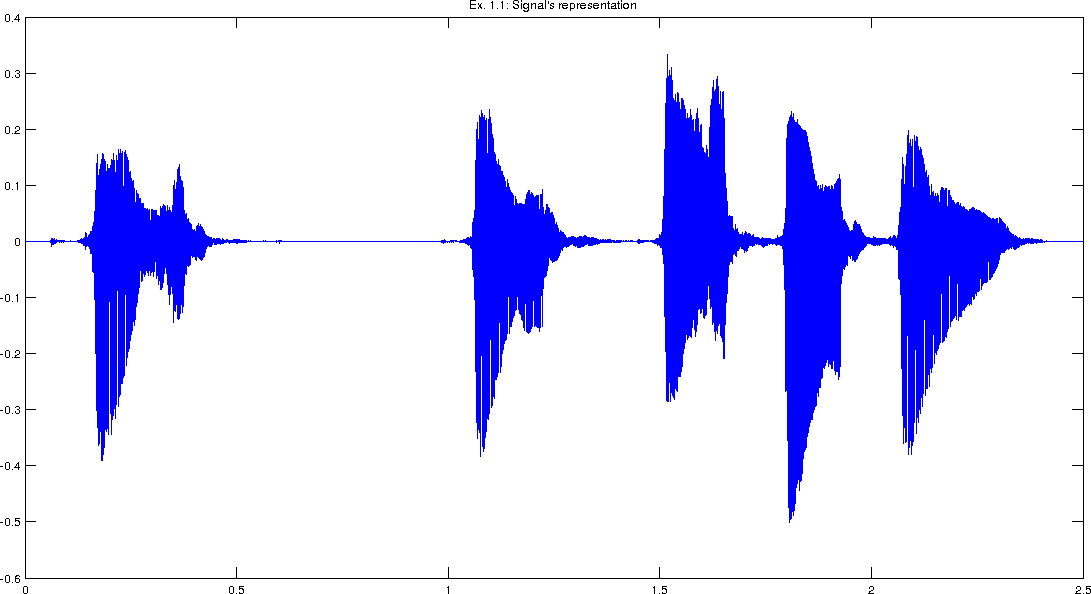
\includegraphics[width=0.65\textwidth]{images/ex_1_1_sign.png}
	\captionof{figure}{Signal''s representation}
\end{center}

\begin{center}
	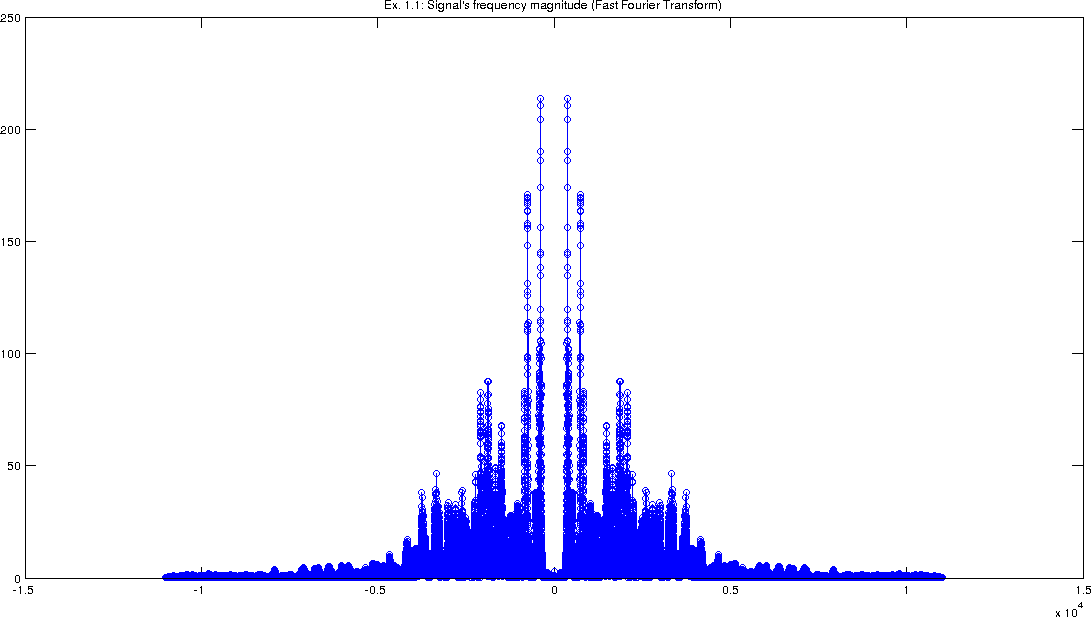
\includegraphics[width=0.65\textwidth]{images/ex_1_1_mag.png}
	\captionof{figure}{Signal's frequency magnitude (Fast Fourier Transform)}
\end{center}

\subsection{Exercise 1.2 - 1.4}
\indent \indent Representa-se a janela de \emph{Hamming} utilizada em função frequência.
\begin{center}
	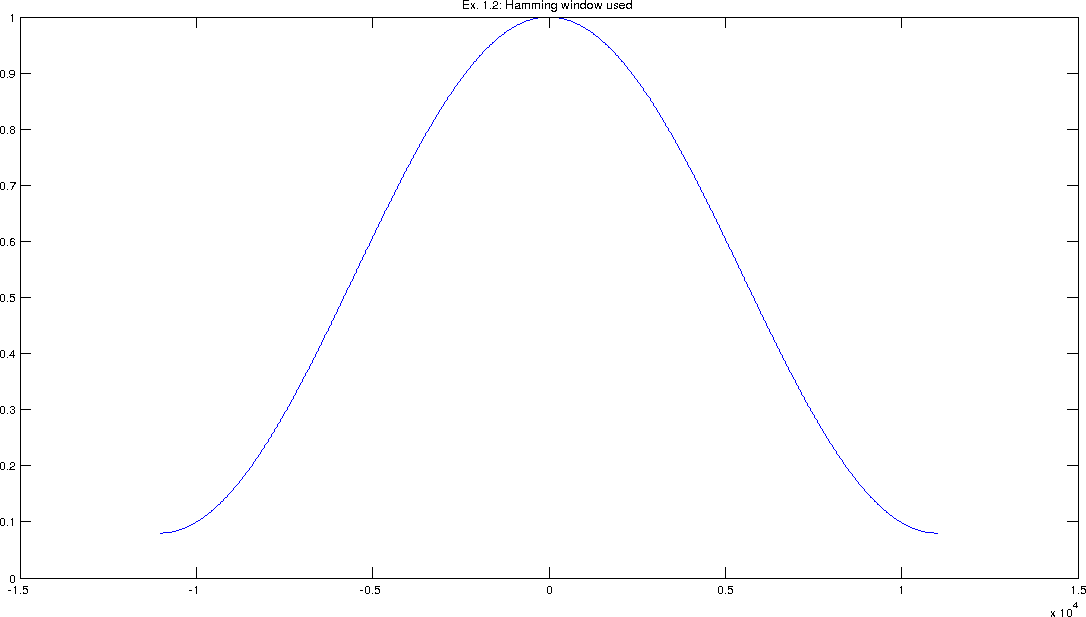
\includegraphics[width=0.65\textwidth]{images/ex_1_2_hamming.png}
	\captionof{figure}{Hamming window}
\end{center}

Utilizando a função \emph{stairs} para representar a sequência de frequências fundamentais (consideradas como sendo as frequências de amplitude máxima de frequência superior a 100 Hz), apresentam-se os gráficos para uma mediana de 1 (original), 5, 7 e 9, juntamente com a representação gŕafica dos sinais sintetizados a partir dessas mesmas sequências.

\subsubsection{Mediana 1}
\begin{center}
	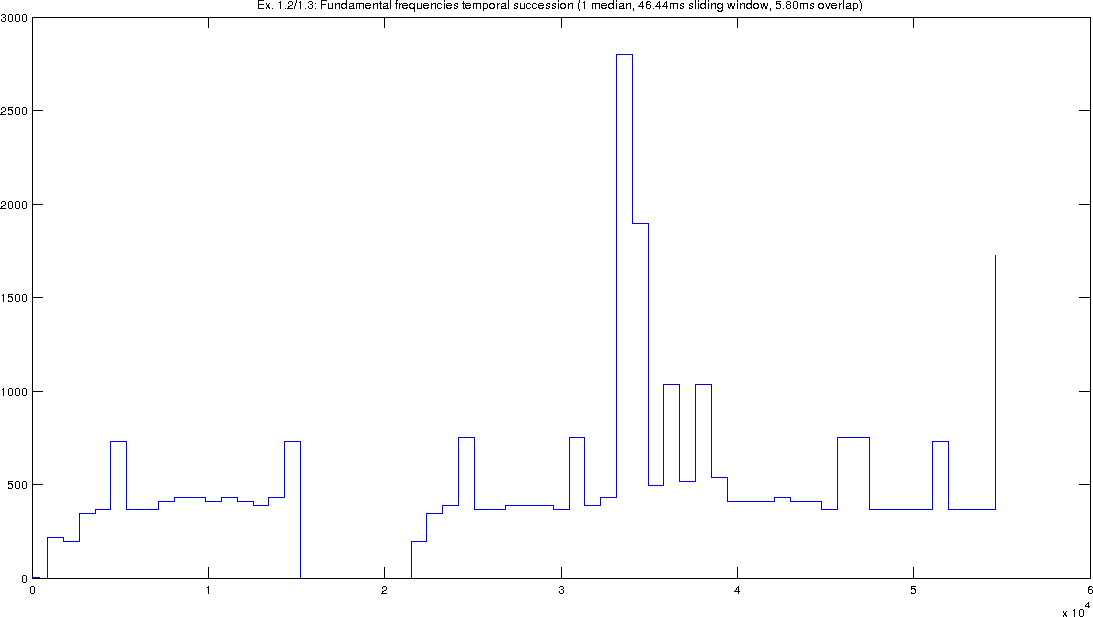
\includegraphics[width=0.65\textwidth]{images/ex_1_3_succession_1.png}
	\captionof{figure}{Fundamental frequencies temporal succession 1 median, 46.44ms sliding window, 5.80ms overlap.}
\end{center}
\begin{center}
	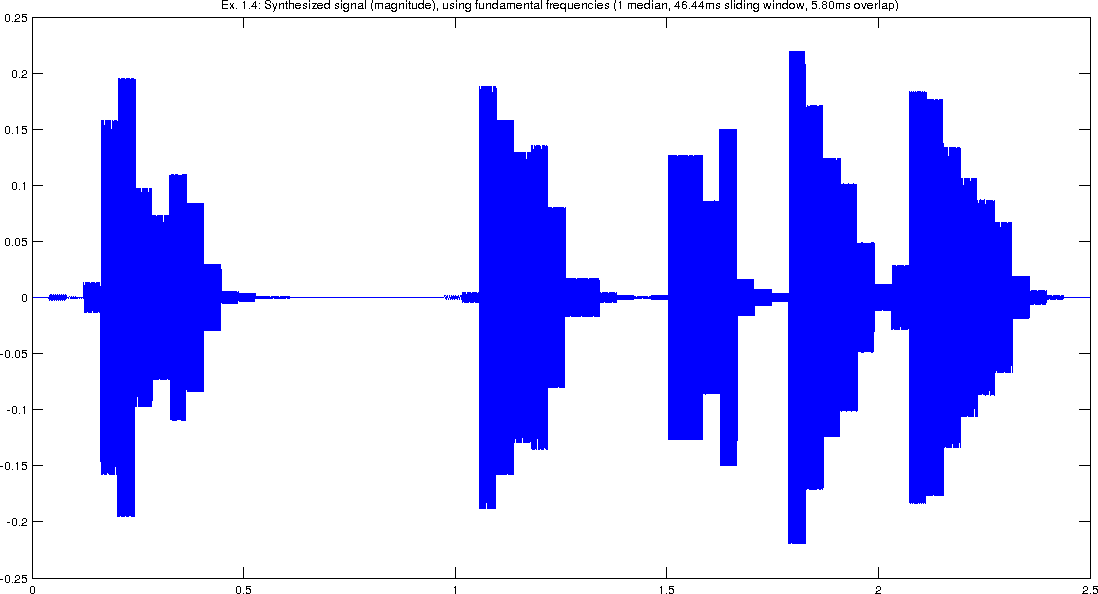
\includegraphics[width=0.65\textwidth]{images/ex_1_4_synth_1.png}
	\captionof{figure}{Synthesized signal (magnitude), using fundamental frequencies 1 median, 46.44ms sliding window, 5.80ms overlap.}
\end{center}

\subsubsection{Mediana 5}
\begin{center}
	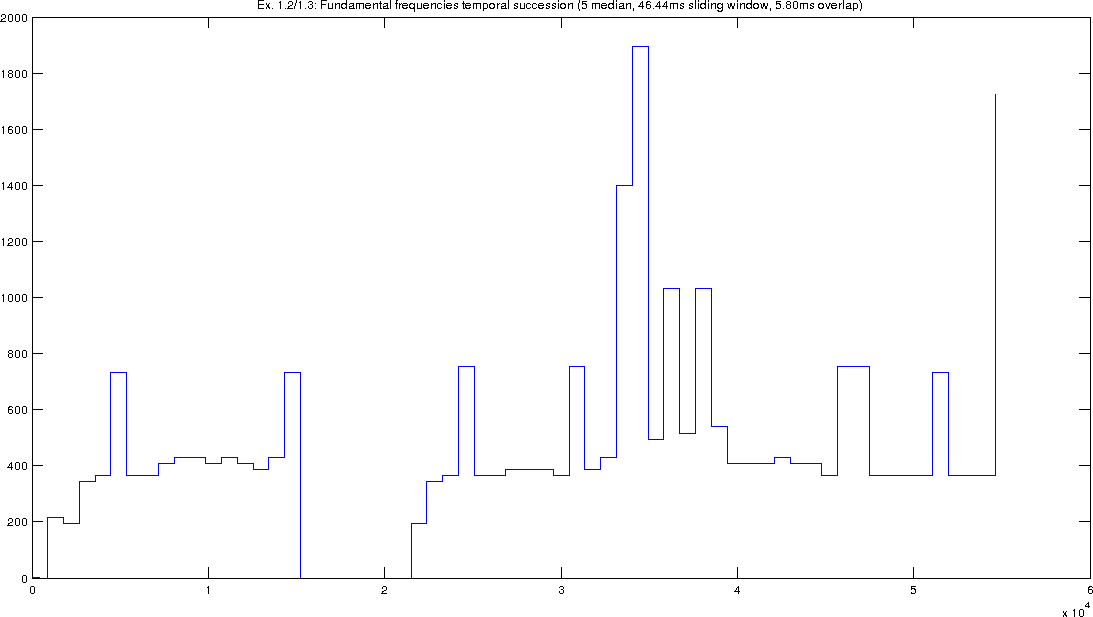
\includegraphics[width=0.65\textwidth]{images/ex_1_3_succession_5.png}
	\captionof{figure}{Fundamental frequencies temporal succession 5 median, 46.44ms sliding window, 5.80ms overlap.}
\end{center}
\begin{center}
	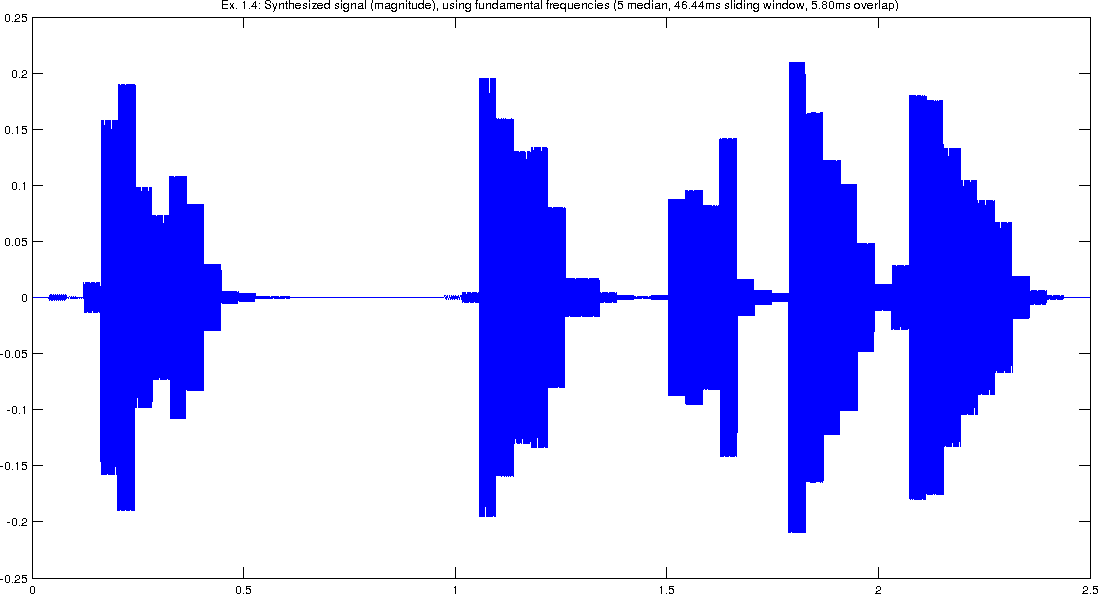
\includegraphics[width=0.65\textwidth]{images/ex_1_4_synth_5.png}
	\captionof{figure}{Synthesized signal (magnitude), using fundamental frequencies 5 median, 46.44ms sliding window, 5.80ms overlap.}
\end{center}

\subsubsection{Mediana 7}
\begin{center}
	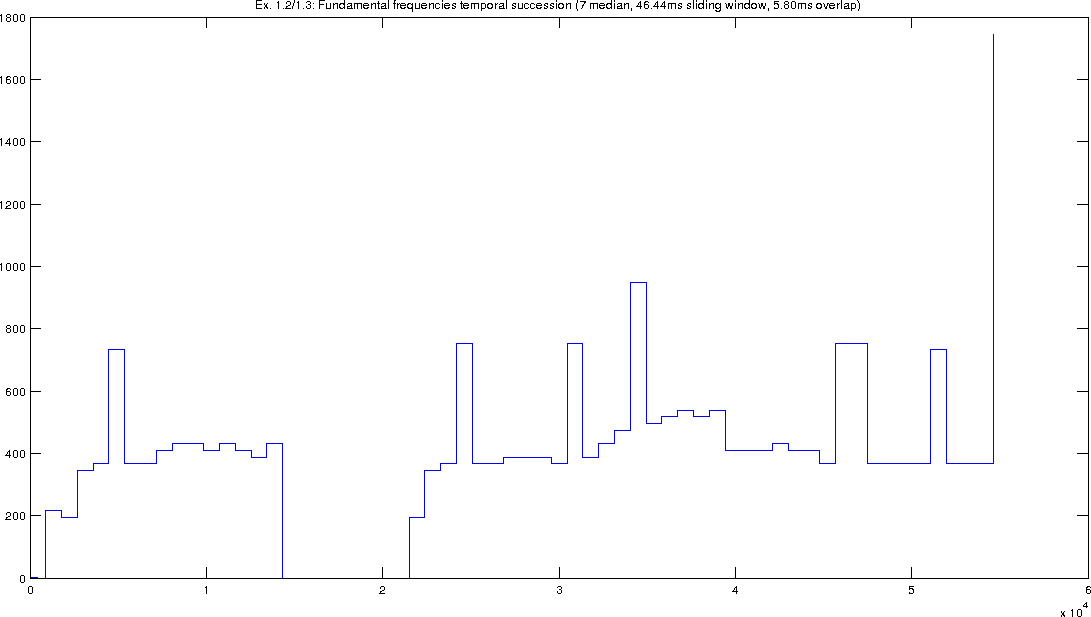
\includegraphics[width=0.65\textwidth]{images/ex_1_3_succession_7.png}
	\captionof{figure}{Fundamental frequencies temporal succession 7 median, 46.44ms sliding window, 5.80ms overlap.}
\end{center}
\begin{center}
	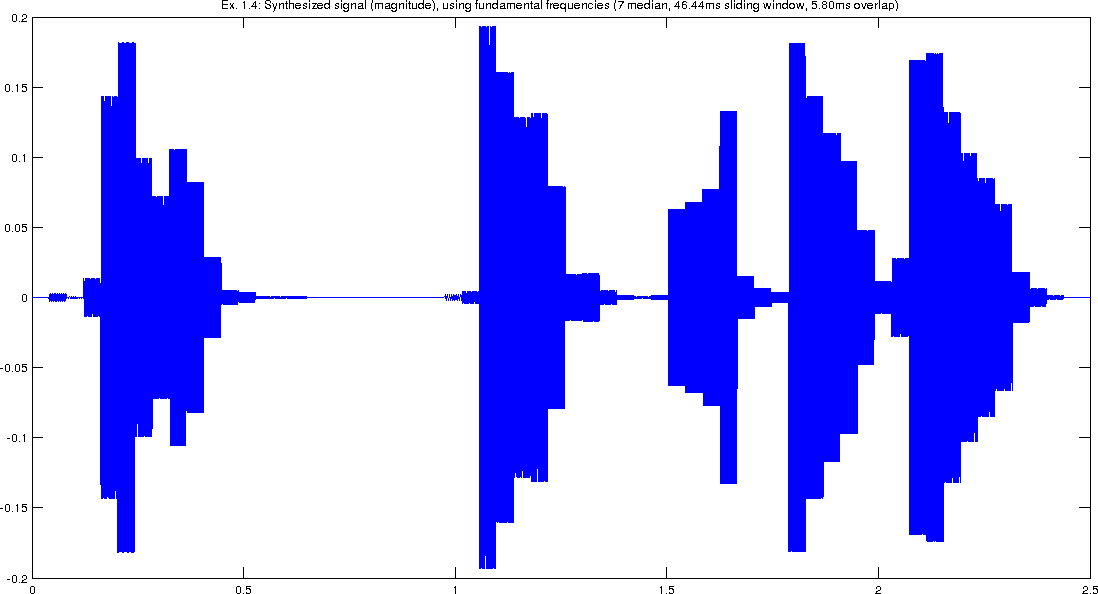
\includegraphics[width=0.65\textwidth]{images/ex_1_4_synth_7.png}
	\captionof{figure}{Synthesized signal (magnitude), using fundamental frequencies 7 median, 46.44ms sliding window, 5.80ms overlap.}
\end{center}

\subsubsection{Mediana 9}
\begin{center}
	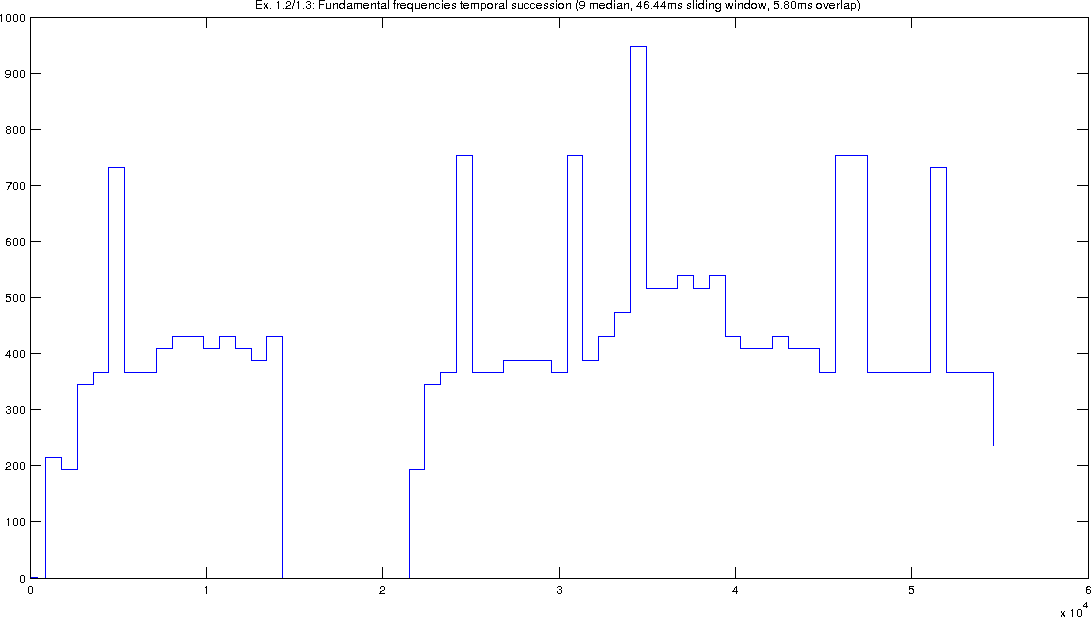
\includegraphics[width=0.65\textwidth]{images/ex_1_3_succession_9.png}
	\captionof{figure}{Fundamental frequencies temporal succession 9 median, 46.44ms sliding window, 5.80ms overlap.}
\end{center}
\begin{center}
	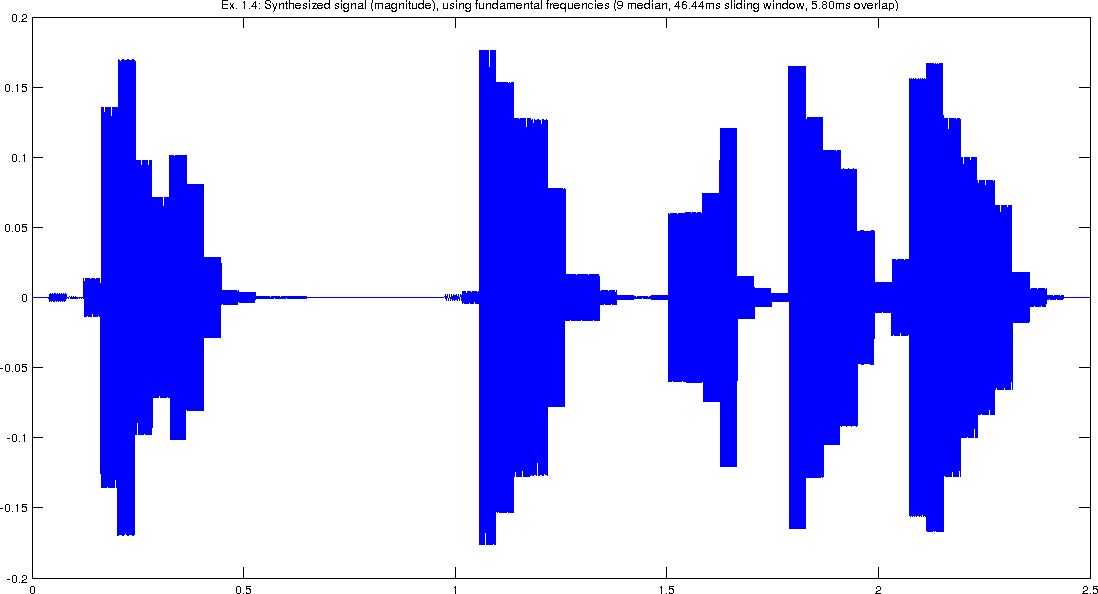
\includegraphics[width=0.65\textwidth]{images/ex_1_4_synth_9.png}
	\captionof{figure}{Synthesized signal (magnitude), using fundamental frequencies 9 median, 46.44ms sliding window, 5.80ms overlap.}
\end{center}

\subsection{Exercise 1.5}
\indent \indent Nota-se que os sinais sintetizadas possuem as principais notas do sinal original, parecendo que este foi ``discretizado''. Entre os vários sinais sintetizados, é possível verificar que os sons com maior mediana vão perdendo intensidade nalguns picos de frequência altas, ficando o sinal mais suave em termos de volume e percepção.

\section{Exercise 2}
\subsection{Exercise 2.1 - 2.4}
\indent \indent Apresenta-se em seguida a representação gráfica de cada sinal, a representação da magnitude do espectro em função da frequência, bem como os valores considerados para a duração da janela, sobreposição, resolução temporal obtida com esses valores e sequência temporal de notas obtida.

\subsubsection{\texttt{escala.wav}}
\begin{center}
	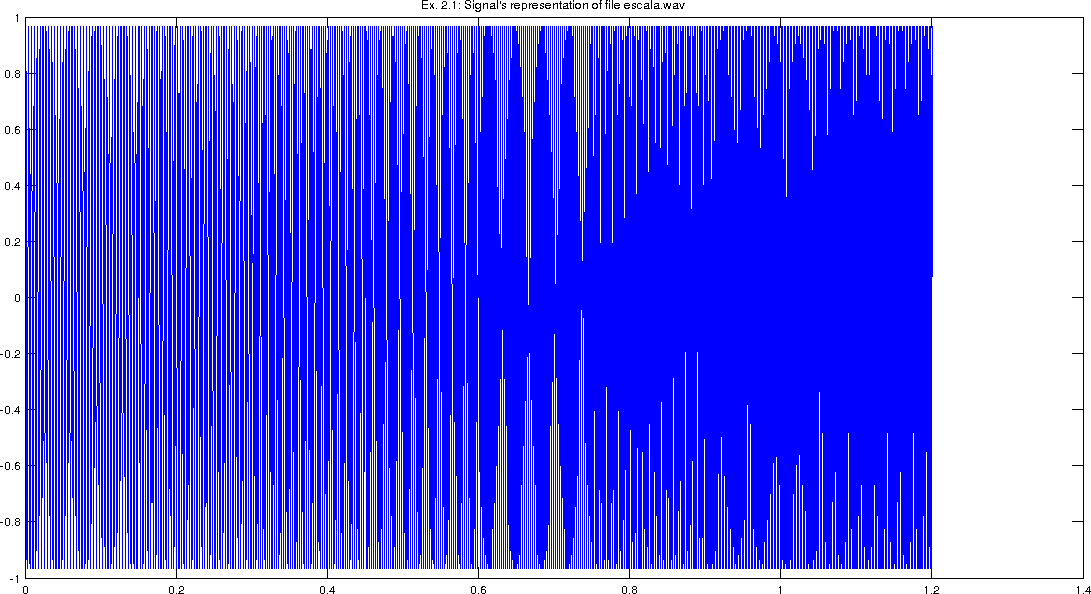
\includegraphics[width=0.65\textwidth]{images/ex_2_1_escala_sign.png}
	\captionof{figure}{Signal''s representation of file escala.wav.}
\end{center}
\begin{center}
	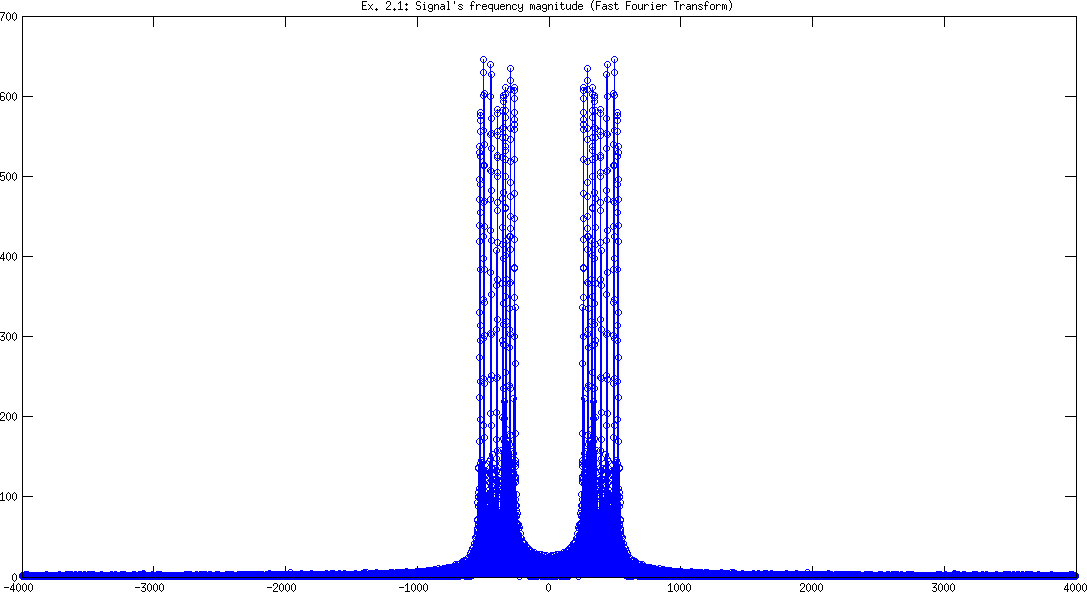
\includegraphics[width=0.65\textwidth]{images/ex_2_1_escala_mag.png}
	\captionof{figure}{Signal''s frequency magnitude (Fast Fourier Transform).}
\end{center}

\indent \indent Considerámos para este sinal uma janela de duração 150ms, com sobreposição de 4.69ms. Como tal, obtemos uma resolução em frequência de 6.67Hz. Apresenta-se em seguida a sequência temporal de notas obtida (graficamente e textualmente).
\begin{center}
	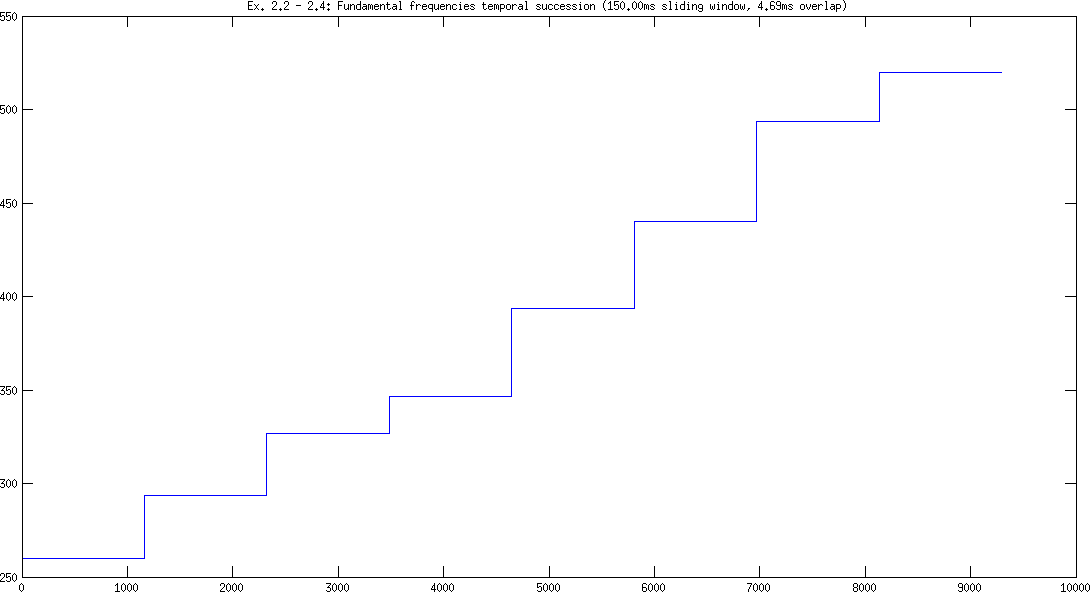
\includegraphics[width=0.65\textwidth]{images/ex_2_2_escala.png}
	\captionof{figure}{Fundamental frequencies temporal succession (150.00ms sliding window, 4.69ms overlap).}
\end{center}

Do Re Mi Fa Sol La Si Do Do

\subsubsection{\texttt{piano.wav}}
\begin{center}
	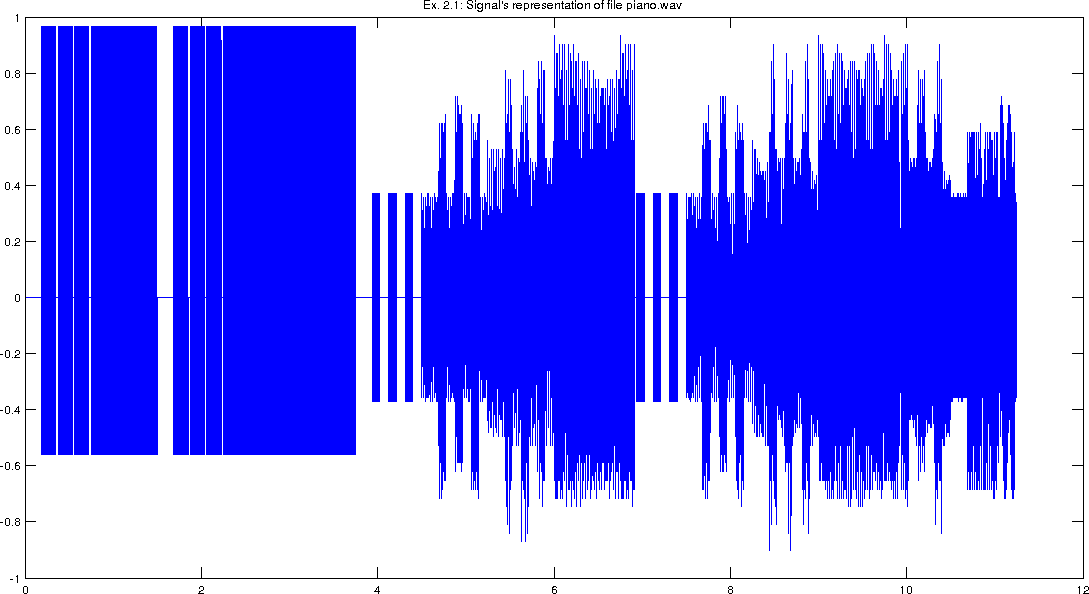
\includegraphics[width=0.65\textwidth]{images/ex_2_1_piano_sign.png}
	\captionof{figure}{Signal''s representation of file piano.wav.}
\end{center}
\begin{center}
	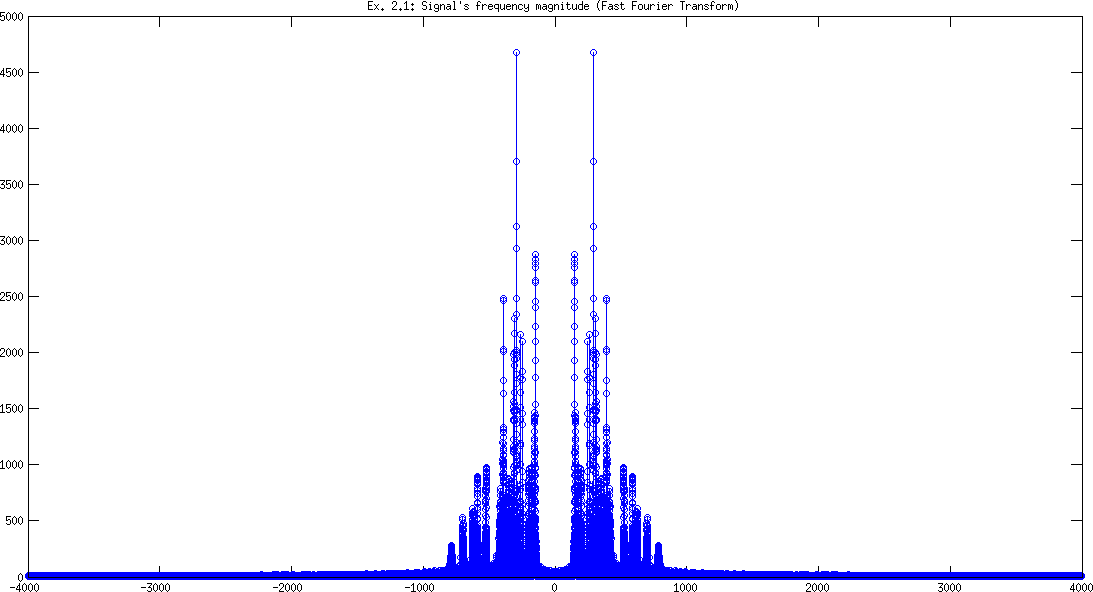
\includegraphics[width=0.65\textwidth]{images/ex_2_1_piano_mag.png}
	\captionof{figure}{Signal''s frequency magnitude (Fast Fourier Transform).}
\end{center}

\indent \indent Considerámos para este sinal uma janela de duração 180ms, com sobreposição de 5.62ms. Como tal, obtemos uma resolução em frequência de 5.56Hz. Apresenta-se em seguida a sequência temporal de notas obtida (graficamente e textualmente).
\begin{center}
	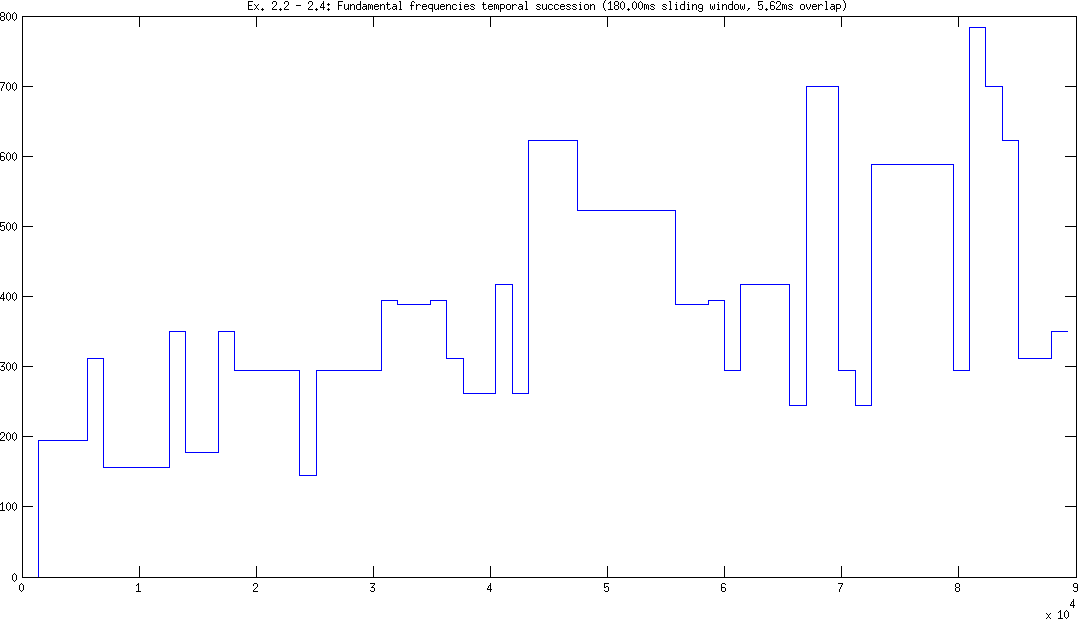
\includegraphics[width=0.65\textwidth]{images/ex_2_2_piano.png}
	\captionof{figure}{Fundamental frequencies temporal succession (180.00ms sliding window, 5.62ms overlap).}
\end{center}

. Sol Sol Sol Re\# Re\# Re\# Re\# Re\# Fa Fa Fa Fa Re Re Re Re Re Re Re Re Re Sol Sol Sol Sol Re\# Do Do Sol\# Do Re\# Re\# Re\# Do Do Do Do Do Do Sol Sol Sol Re Sol\# Sol\# Sol\# Si Fa Fa Re Si Re Re Re Re Re Re Sol Fa Re\# Re\# Re\# Fa Fa

\subsubsection{\texttt{flauta.wav}}
\begin{center}
	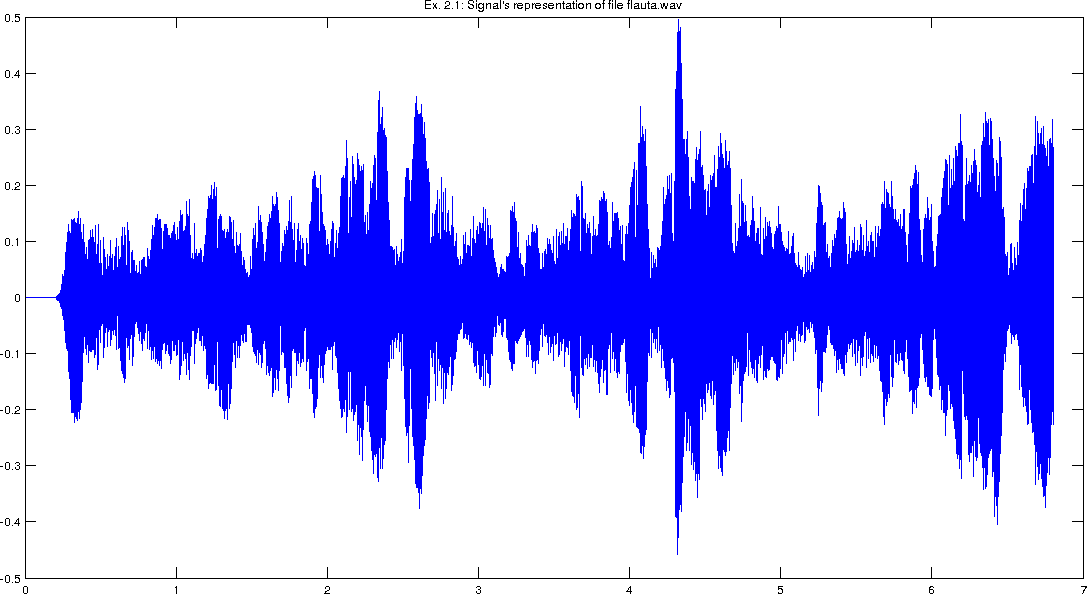
\includegraphics[width=0.65\textwidth]{images/ex_2_1_flauta_sign.png}
	\captionof{figure}{Signal''s representation of file flauta.wav.}
\end{center}
\begin{center}
	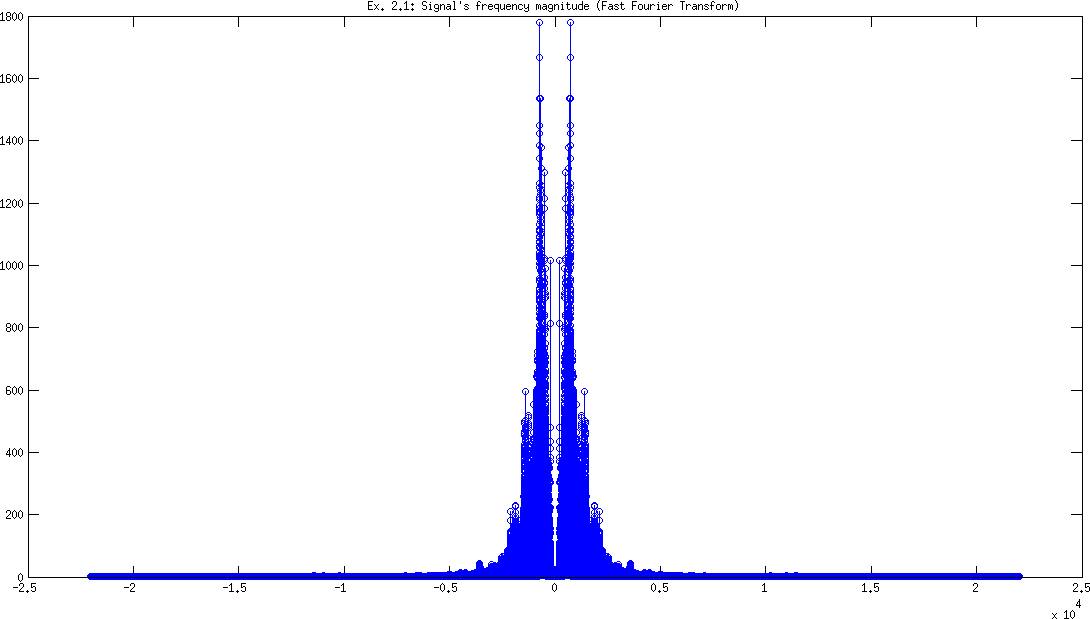
\includegraphics[width=0.65\textwidth]{images/ex_2_1_flauta_mag.png}
	\captionof{figure}{Signal''s frequency magnitude (Fast Fourier Transform).}
\end{center}

\indent \indent Considerámos para este sinal uma janela de duração 50ms, com sobreposição de 1.56. Como tal, obtemos uma resolução em frequência de 20Hz. Apresenta-se em seguida a sequência temporal de notas obtida (graficamente e textualmente).
\begin{center}
	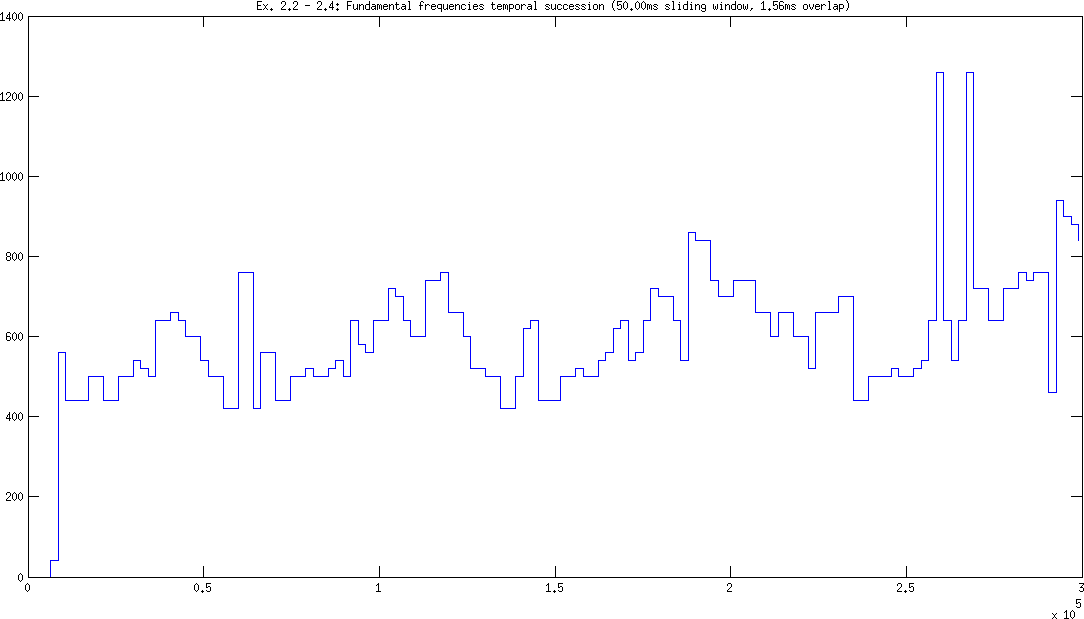
\includegraphics[width=0.65\textwidth]{images/ex_2_2_flauta.png}
	\captionof{figure}{Fundamental frequencies temporal succession (50.00ms sliding window, 1.56ms overlap).}
\end{center}

. . . Re\# Do\# La La La Do Do La La Do Do Do\# Do Do Re\# Re\# Mi Re\# Re Re Do\# Do Do Sol\# Sol\# Fa\# Fa\# Sol\# Do\# Do\# La La Do Do Do Do Do Do Do\# Do Re\# Re Do\# Re\# Re\# Fa\# Fa Re\# Re Re Fa\# Fa\# Fa\# Mi Mi Re Do Do Do Do Sol\# Sol\# Do Re\# Re\# La La La Do Do Do Do Do Do\# Do\# Re\# Re\# Do\# Do\# Re\# Fa\# Fa Fa Re\# Do\# La Sol\# Sol\# Fa\# Fa Fa Fa\# Fa\# Fa\# Mi Mi Re Mi Mi Re Re Do Mi Mi Mi Fa Fa La La Do Do Do Do Do Do Do Do\# Re\# Re\# Re\# Do\# Re\# Re\# Fa\# Fa\# Re\# Re\# Fa\# Fa\# Fa\# Fa\# Fa\# Fa\# La\# La\# La La Sol\# 

\subsection{Exercise 2.5}
\indent \indent A janela escolhida é a mais importante escolha para a correcta identificação das notas, uma vez que essa decide a resolução em frequência obtida. Para os 2 primeiros sinais, a janela foi escolhida de acordo com a duração de cada nota. Dado que são sinais sintetizados com notas igualmente espaçadas (temporalmente), a janela é relativamente fácil de determinar. Num sinal real (`flauta.wav'), tal escolha torna-se num compromisso, e portanto mais `fine-tuned'.

\section{Exercise 3}
\subsection{Exercise 3.1}
\indent \indent Representa-se de seguida graficamente o sinal `sumsin\_freqbrk'.
\begin{center}
	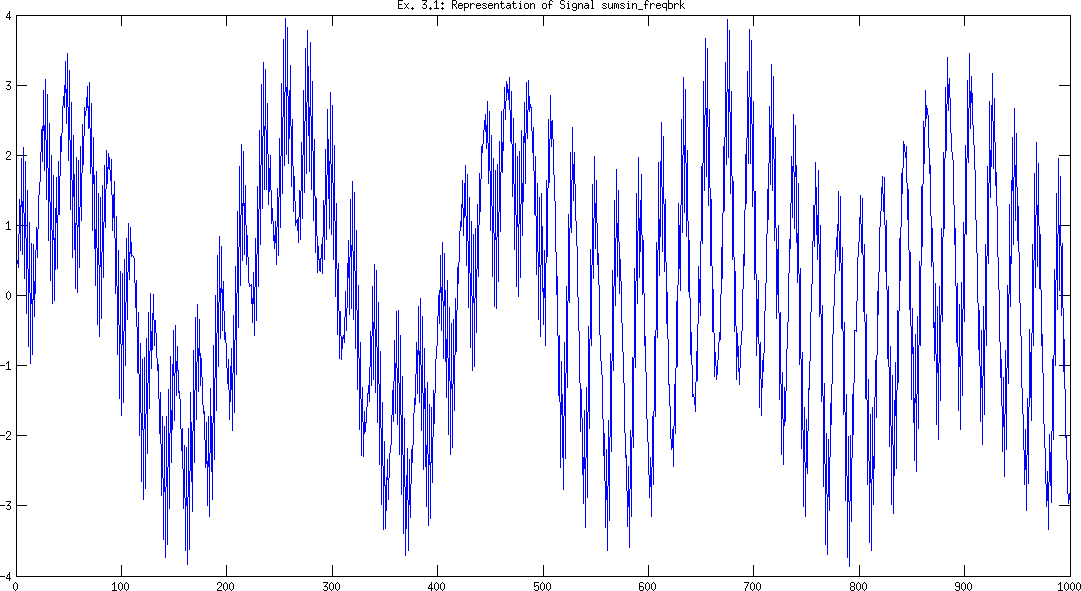
\includegraphics[width=0.65\textwidth]{images/ex_3_1.png}
	\captionof{figure}{Representation of Signal sumsin\_freqbrk.}
\end{center}

\subsection{Exercise 3.2/3.3}
\indent \indent O resultado obtido para a decomposição de um nível do sinal é apresentada abaixo, bem como a reconstrução do mesmo a partir desses coeficientes. Apresenta-se também a sobreposição do sinal original com essa reconstrução, podendo ser verificado serem iguais.
\begin{center}
	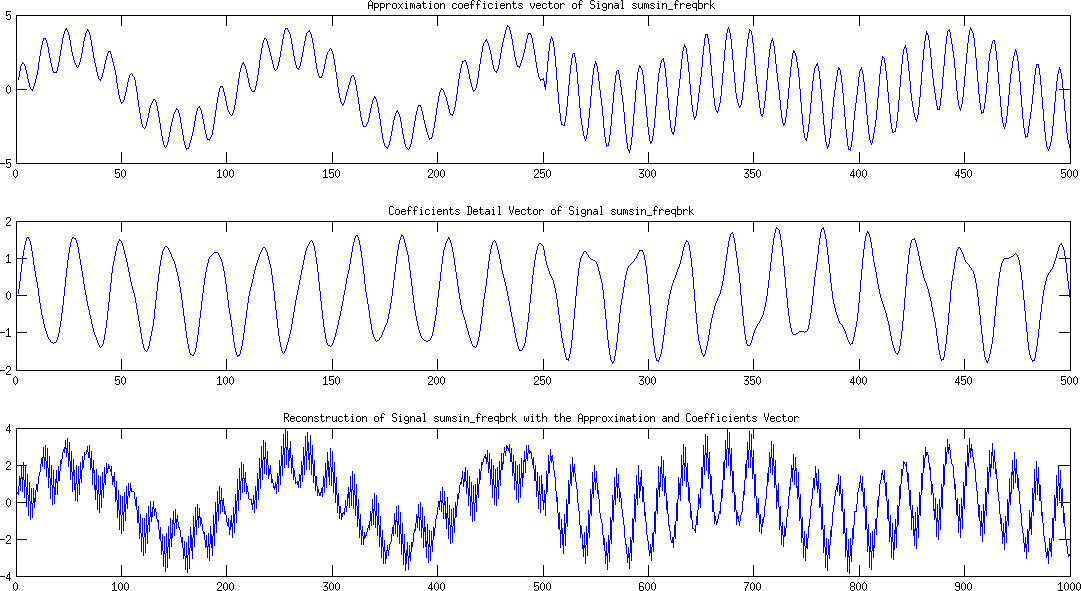
\includegraphics[width=0.65\textwidth]{images/ex_3_2-3.png}
	\captionof{figure}{Representation of approximation coefficients, detail coefficients and the reconstruction of signal.}
\end{center}
\begin{center}
	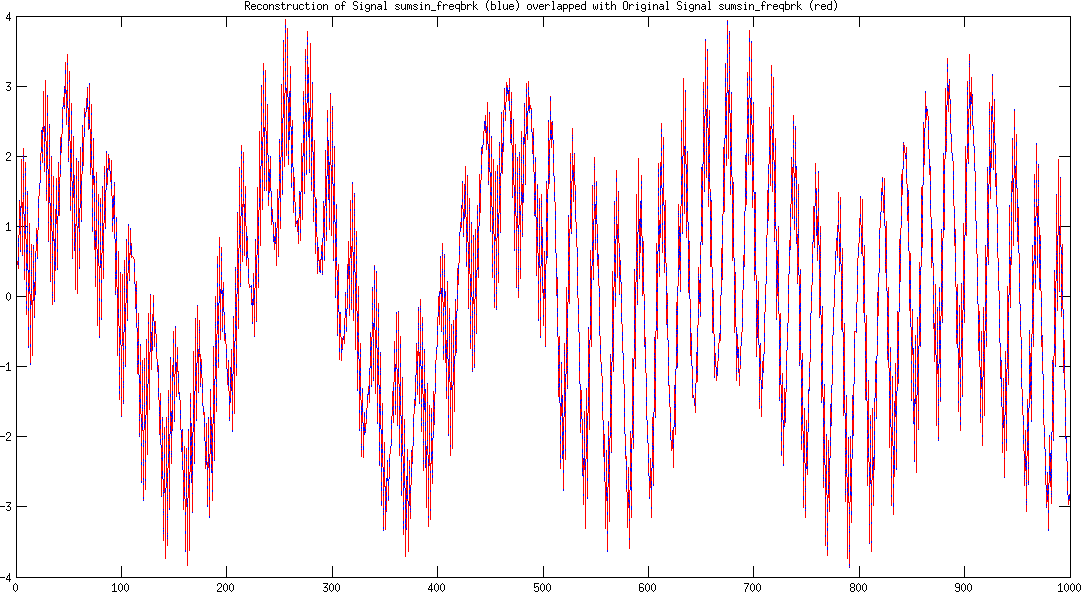
\includegraphics[width=0.65\textwidth]{images/ex_3_3_ep.png}
	\captionof{figure}{Equality of proof: Reconstruction of signal sumsin\_freqbrk (blue) overlapped with original signal (red).}
\end{center}

\subsection{Exercise 3.4}
\indent \indent Apresenta-se os coeficientes (de detalhe e aproximação) resultantes da decomposição do sinal com 4 níveis de resolução, utilizando a \emph{wavelet} `db3'.
\begin{center}
	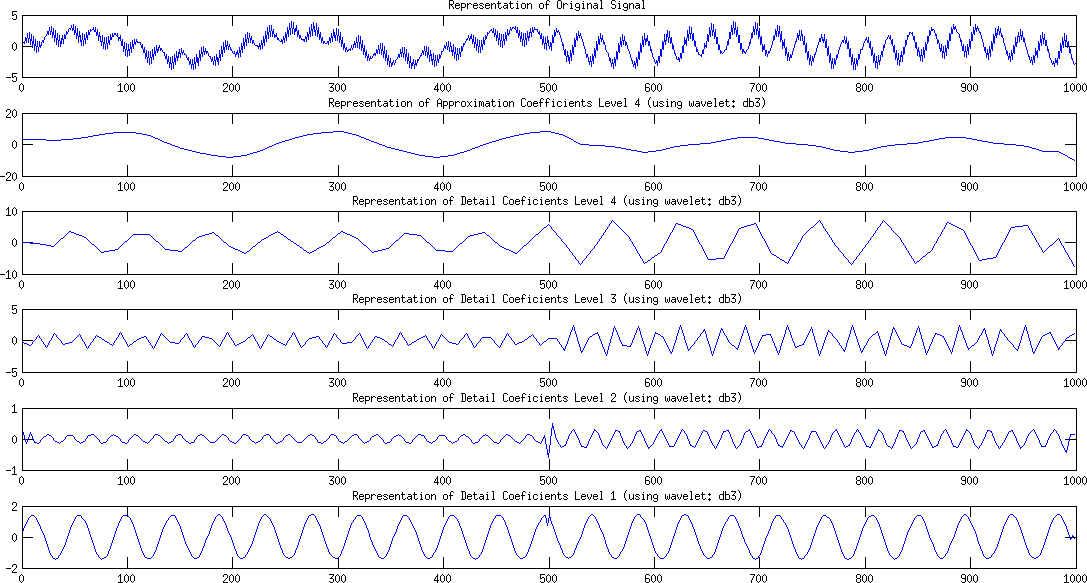
\includegraphics[width=0.85\textwidth]{images/ex_3_4.png}
	\captionof{figure}{Representation of Approximation and Detail Coefficients of using wavelet db3.}
\end{center}

\subsection{Exercise 3.5}
\indent \indent Apresenta-se os coeficientes (de detalhe e aproximação) resultantes da decomposição do sinal com 4 níveis de resolução, utilizando a \emph{wavelet} `sym2'.
\begin{center}
	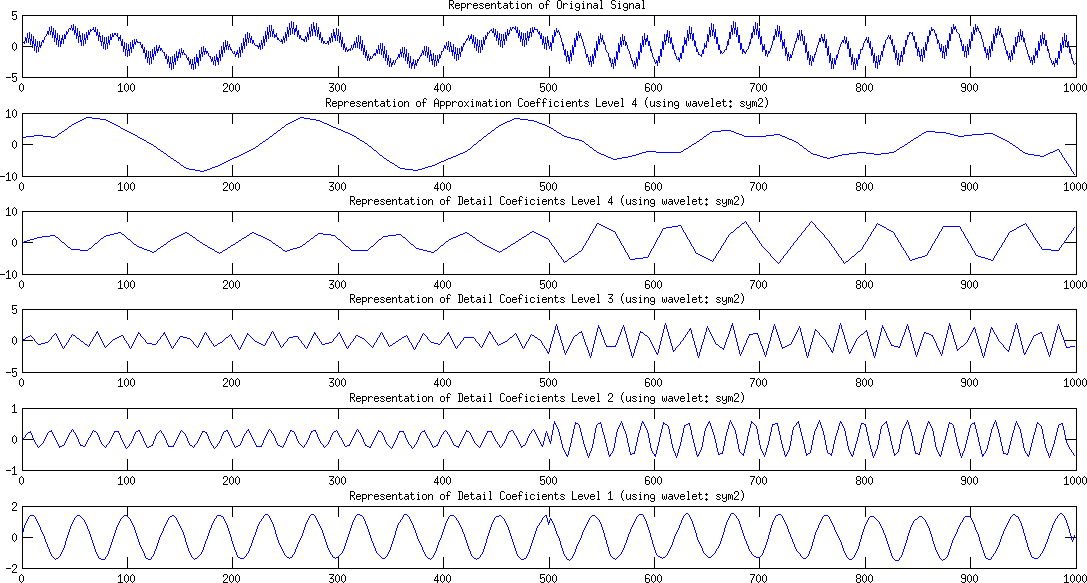
\includegraphics[width=0.85\textwidth]{images/ex_3_5.png}
	\captionof{figure}{Representation of Approximation and Detail Coefficients of using wavelet sym2.}
\end{center}

\subsection{Exercise 3.6}
\indent \indent Apresentam-se em seguida as reconstruções obtidas para as duas \emph{wavelets}, utilizando o coeficiente de aproximação de nível 4, juntamente com os coeficientes de detalhe dos 4 níveis, sobreposta pela reconstrução obtida utilizando a função \texttt{waverec}.

\begin{center}
	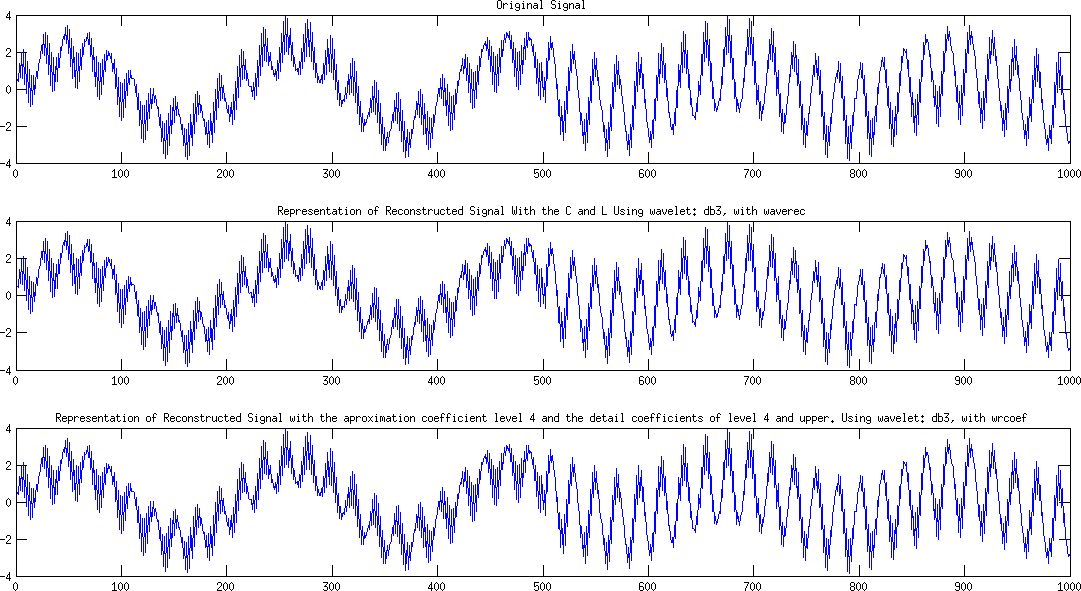
\includegraphics[width=0.85\textwidth]{images/ex_3_6_db3_rec.png}
	\captionof{figure}{Original Signal, Reconstruction of Signal using waverec, Reconstruction of signal using wrcoef (wavelet family: db3).}
\end{center}
\begin{center}
	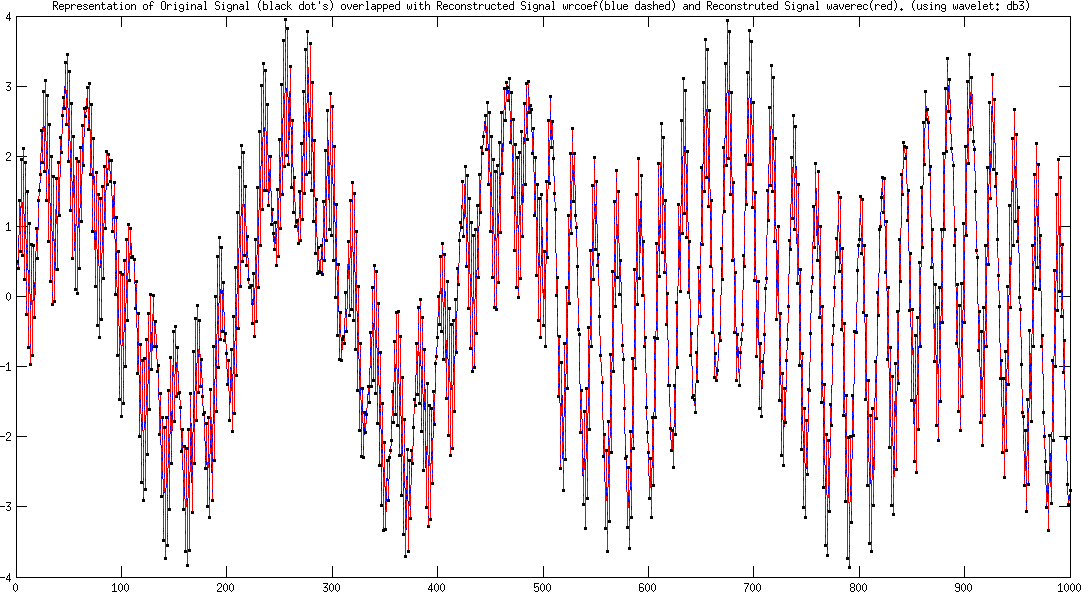
\includegraphics[width=0.85\textwidth]{images/ex_3_6_db3_ep.png}
	\captionof{figure}{Representation of Original Signal (black dot''s) overlapped with Reconstructed Signal wrcoef(blue dashed) and Reconstruted Signal waverec(red). (using wavelet: db3)}
\end{center}

\begin{center}
	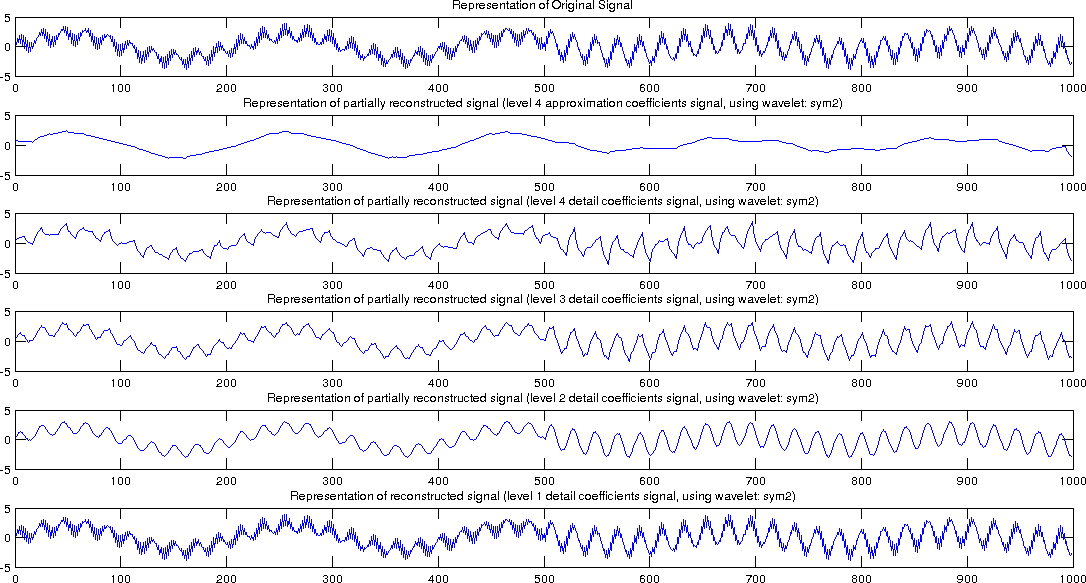
\includegraphics[width=0.85\textwidth]{images/ex_3_6_sym2_rec.png}
	\captionof{figure}{Original Signal, Reconstruction of Signal using waverec, Reconstruction of signal using wrcoef (wavelet family: sym2).}
\end{center}
\begin{center}
	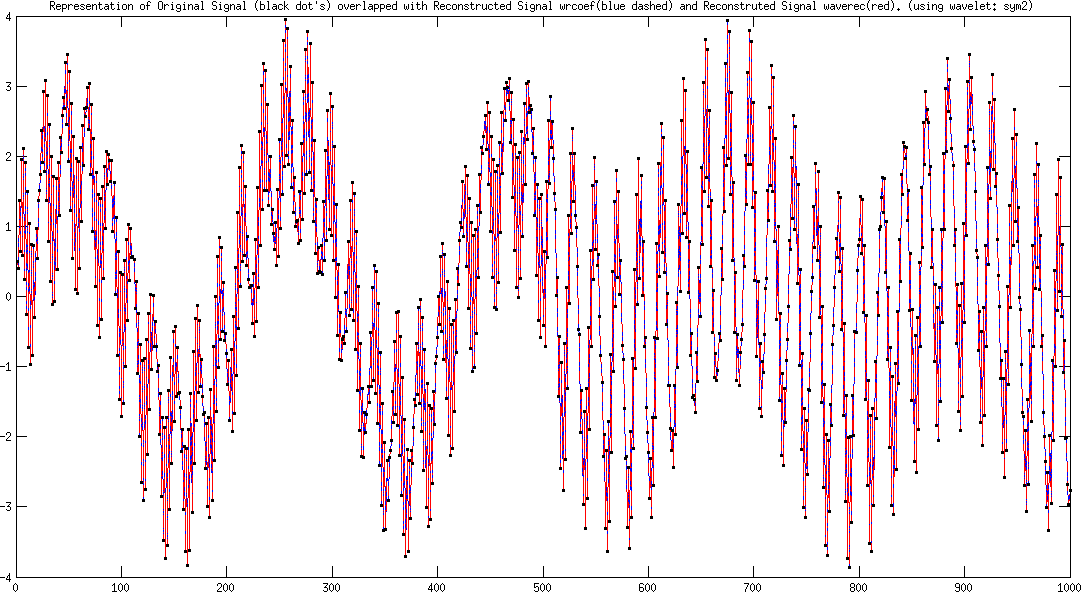
\includegraphics[width=0.85\textwidth]{images/ex_3_6_sym2_ep.png}
	\captionof{figure}{Representation of Original Signal (black dot''s) overlapped with Reconstructed Signal wrcoef(blue dashed) and Reconstruted Signal waverec(red). (using wavelet: sym2)}
\end{center}

\section{Exercise 4}
\subsection{Exercise 4.1}
\indent \indent Decompondo a imagem a dois níveis considerando a \emph{Wavelet de Haar}, obtém-se o resultado apresentado abaixo.
\begin{center}
	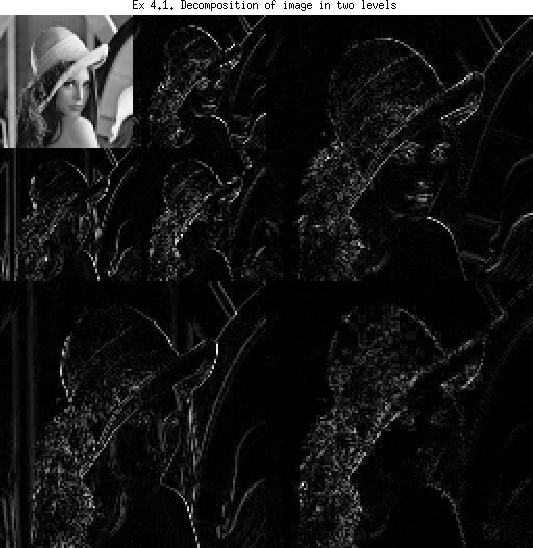
\includegraphics[width=0.65\textwidth]{images/ex_4_1.png}
	\captionof{figure}{Decomposition of image in two levels.}
\end{center}

\subsection{Exercise 4.2}
\indent \indent Apresentamos a reconstrução da imagem obtida utilizando apenas o coeficiente de detalhe de nível 2, detalhe de nível 1 e todos.
\begin{center}
	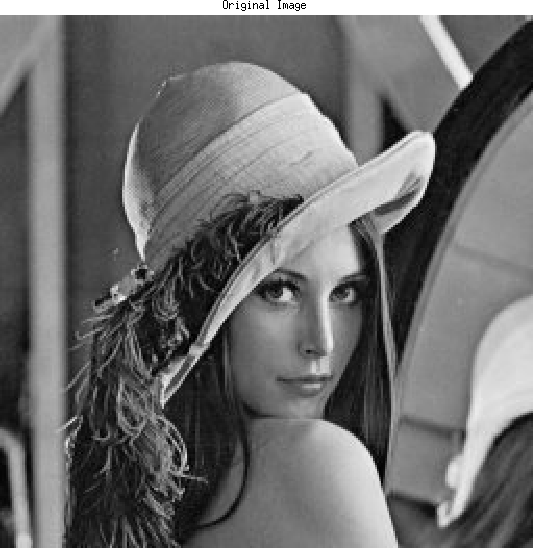
\includegraphics[width=0.50\textwidth]{images/ex_4_2_original.png}
	\captionof{figure}{Original Image}
\end{center}
\begin{center}
	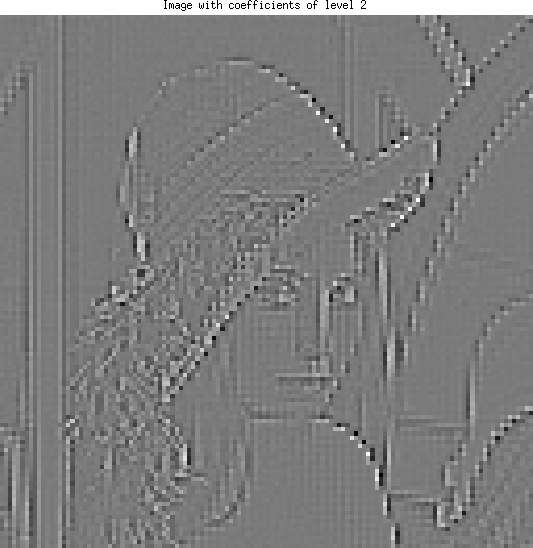
\includegraphics[width=0.50\textwidth]{images/ex_4_2_coef_l2.png}
	\captionof{figure}{Image with detail coefficients of level 2.}
\end{center}
\begin{center}
	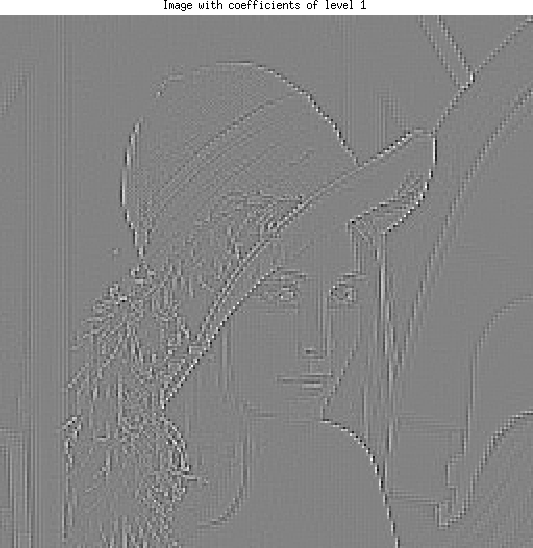
\includegraphics[width=0.50\textwidth]{images/ex_4_2_coef_l1.png}
	\captionof{figure}{Image with detail coefficients of level 1.}
\end{center}
\begin{center}
	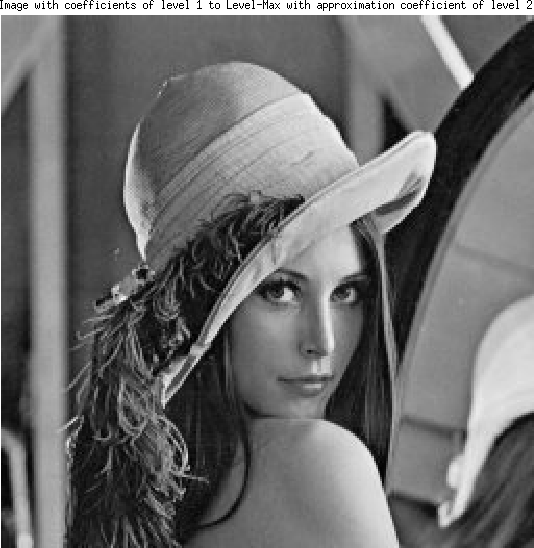
\includegraphics[width=0.50\textwidth]{images/ex_4_2_all_coef.png}
	\captionof{figure}{Image with detail coefficients of level 1 and 2 with approximation coefficient of level 2.}
\end{center}
\end{document}
